% Problem Set 8 -- Question (g) and AI Integration. Place this file and both
% ps8_tstat_*.png images next to the final report's main .tex file.
% Requires graphicx and booktabs. All Sharpe comparisons use monthly units.

\subsection*{Question (g): Random strategies}

We simulated 5,000 strategies, drawing one of the 75 portfolios independently
for each month and strategy, with replacement (seed 20261105). We used monthly
returns in excess of the T-bill and excluded $-999$ and $-99.99$ missing
codes. The common sample has 1,124 months between February 1931 and June 2026;
21 months in this interval were dropped because at least one portfolio return
was missing. For each strategy we computed its mean, sample standard deviation,
Sharpe ratio and $t$-statistic, $t=\sqrt{T}\,\bar r/s$.

\begin{table}[htbp]
\centering\small
\caption{5,000 random strategies, full common sample ($T=1{,}124$). Returns and standard deviations are monthly.}
\label{tab:gfull}
\begin{tabular}{lrr}
\toprule
 & Raw excess returns & Demeaned excess returns\\
\midrule
Average mean return (\%) & 0.7975 & 0.0012\\
Average standard deviation (\%) & 6.5092 & 6.5024\\
Average monthly Sharpe & 0.1225 & 0.0001\\
Average annualized Sharpe & 0.4244 & 0.0002\\
Average $t$-statistic & 4.107 & 0.002\\
Number with $t>2$ / $t<-2$ & 5,000 / 0 & 0 / 0\\
Fraction with $|t|>2$ (\%) & 100.00 & 0.00\\
Fraction with two-sided $p<0.05$ (\%) & 100.00 & 0.00\\
\bottomrule
\end{tabular}
\end{table}

All 5,000 raw strategies have $t>2$ (Figure~\ref{fig:g-hist}, left). This does not mean that random
portfolio switching creates alpha: the underlying portfolios earn positive
excess returns. Under a true independent normal zero-mean null, roughly 5\%
of conventional two-sided tests would reject at the 5\% level, but that is
\emph{not} the expected rate for these positive-premium, correlated portfolios.

To separate this effect from chance findings, we subtracted each portfolio's
mean over the same 1,124 months and repeated the same 5,000 draws. No demeaned
strategy has $|t|>2$ (Figure~\ref{fig:g-hist}, right). This 0\% result is valid even though it is below the
usual 5\% benchmark. Since each portfolio has zero sample mean, the average
across portfolios and then across all months is exactly zero. Much of their
remaining volatility comes from shared monthly market movements (mean
pairwise correlation 0.84), but those movements cannot increase the average
return of the randomly switched strategy. Hence its conventional $t$-statistics
are tightly concentrated (SD 0.424), rather than having SD near one. In a
\emph{separate} diagnostic that also resamples months, 4.84\% have $|t|>2$
(5.32\% have $p<0.05$). That diagnostic is not the assigned experiment.
The raw extremes therefore mostly reflect existing premia, not 5,000
independent discoveries of alpha; the simulated strategies also share the
same market history.



\begin{figure}[htbp]
\centering
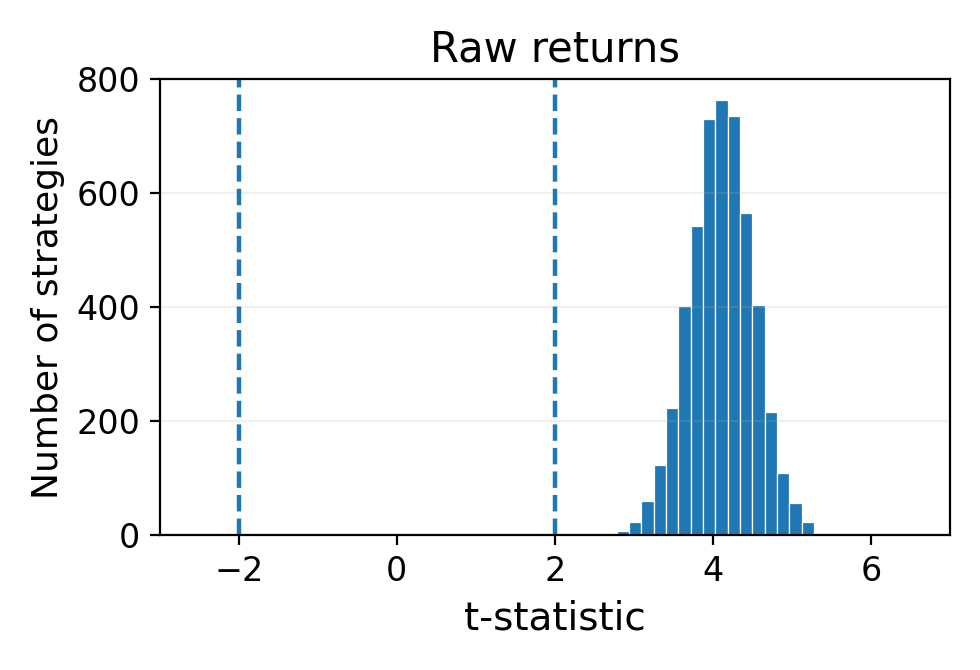
\includegraphics[width=.49\linewidth]{ps8_tstat_raw.png}\hfill
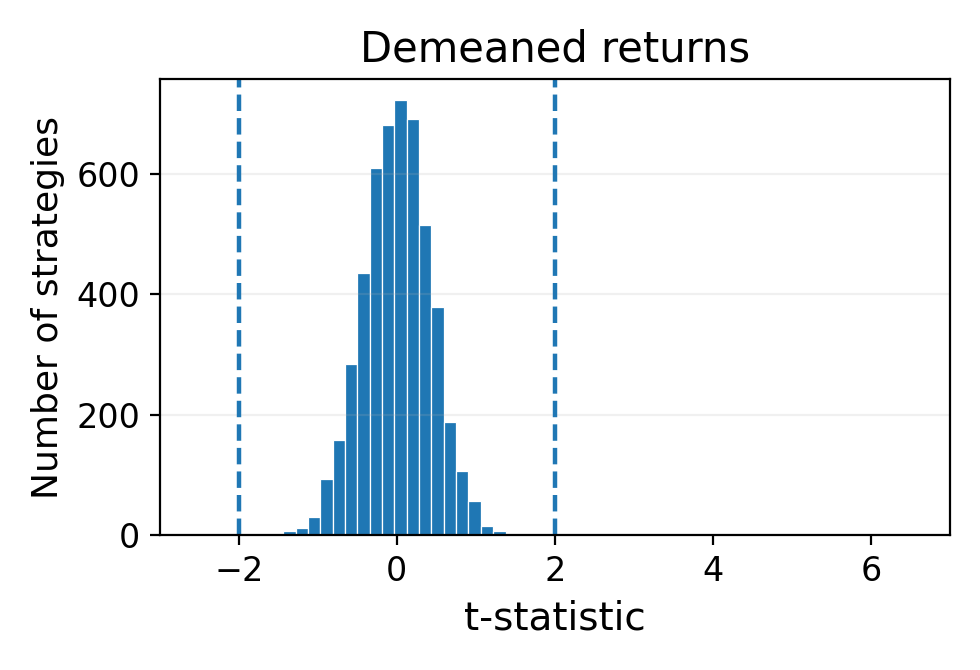
\includegraphics[width=.49\linewidth]{ps8_tstat_demeaned.png}
\caption{Full-sample $t$-statistics before and after portfolio-level demeaning.
Dashed reference lines are $-2$ and $+2$.}
\label{fig:g-hist}
\end{figure}

\paragraph{Comparison with the strategy from (e).}
We compared the random strategies with (e) over exactly the months that (e)
covers: the walk-forward training period (March 1953--June 2001, $T=580$) and
the held-out test period (July 2001--June 2026, $T=300$). In each window we drew
5,000 new random strategies with the same seed. The random strategies are not
charged trading costs, so comparing them only with the \emph{net} returns of (e)
would be unbalanced; Table~\ref{tab:gcompare} reports the gross comparison as
well. The CI limits are the 95\% intervals from (f), converted to monthly
Sharpe units.

\begin{table}[htbp]
\centering\small
\caption{Fraction of the 5,000 raw random strategies in each window whose Sharpe ratio exceeds that of the strategy in (e) or the upper end of its 95\% CI from (f). Random strategies have no trading-cost deductions.}
\label{tab:gcompare}
\begin{tabular}{llrrrr}
\toprule
Sample & (e) returns & Monthly SR & Annual SR & Beat (e) SR & Beat upper 95\% CI\\
 & & & & (\%) & Normal / General (\%)\\
\midrule
Training, 1953--2001 & Gross & 0.4429 & 1.5343 & 0.00 & 0.00 / 0.00\\
($T=580$) & Net & 0.3858 & 1.3365 & 0.00 & 0.00 / 0.00\\
\addlinespace
Test, 2001--2026 & Gross & 0.0996 & 0.3449 & 94.12 & 0.08 / 0.06\\
($T=300$) & Net & 0.0312 & 0.1081 & 100.00 & 39.94 / 40.04\\
\bottomrule
\end{tabular}
\end{table}

In the training window the average random strategy has a monthly Sharpe ratio
of 0.1370 (0.4746 annualized), and the highest is 0.203, below even the lowest
CI limit for (e), 0.290 (net, general). In the test window the average is
0.1379 (0.4778 annualized), and 81.94\% of random strategies have $|t|>2$
(84.12\% have $p<0.05$). The test CI upper limits are 0.2130 (normal) and
0.2133 (general) gross, and 0.14439 and 0.14436 net. Demeaning within the test
window makes only 10.8\% of random strategies beat the net SR of 0.0312, and
none beat the gross SR of 0.0996. This is a sensitivity check, \emph{not} a
risk-matched alternative, because it removes the premia from the random
portfolios but not from (e).

The comparison is not apples-to-apples. The random strategies are long-only
and benefit from the positive equity premia in the underlying portfolios.
The strategy in (e) is long seven portfolios and short seven with zero net
dollar exposure, which may reduce its market exposure but does not eliminate
systematic risk. The gap in Sharpe ratios therefore does not directly tell us whether the signals in (e)
are better or worse than random selection. The training-period comparison
is also biased in favor of (e): it combines several signals chosen from
full-sample results in (a), (b) and (d), and the rule was revised after earlier
test results had been viewed. The one-rule random strategies have no such
search behind them, so (e) beating all of them in training overstates its
merit. Its strong training and weak test performance illustrate selection
risk, not a clean, independently validated anomaly.

\paragraph{Bonus.}
The question does not fix the sample. We read ``the backtested Sharpe ratio''
as the one from the training period on which the rule was built, so our main
calculation uses the net walk-forward training returns (March 1953--June 2001,
$T=580$); the test period is reported briefly below. The largest monthly net
excess return is $+24.02\%$ (February 2000) and the smallest is $-17.06\%$
(March 2000). The mean is 1.243\% and the standard deviation 3.221\% per month,
so the monthly Sharpe ratio is 0.3858 (1.3365 annualized), and the two extremes
lie 7.07 and 5.68 standard deviations from the mean.

\emph{(a) Backtested Sharpe ratio taken as true.} We model monthly returns as
normal with standard deviation $\sigma$ equal to the sample value and mean
$\widehat{SR}\cdot\sigma$. A month at least as high as $+24.02\%$ then has
probability $7.7\times10^{-13}$, and a month at least as low as $-17.06\%$ has
probability $6.6\times10^{-9}$. Over 580 independent months, the chance of at
least one such month is $4.5\times10^{-10}$ and $3.9\times10^{-6}$.

\emph{(b) Any Sharpe ratio in the 95\% CI.} Holding $\sigma$ fixed and letting
the true Sharpe ratio range over the training interval from (f), the
upper-tail probability is between $4.2\times10^{-13}$ and $1.4\times10^{-12}$
for the normal interval (1.04 to 1.63 annualized) and between
$3.8\times10^{-13}$ and $1.5\times10^{-12}$ for the general interval (1.00 to
1.67). The lower-tail probability is between $4.0\times10^{-9}$ and
$1.1\times10^{-8}$ (normal) and between $3.8\times10^{-9}$ and
$1.2\times10^{-8}$ (general). A higher Sharpe ratio makes the maximum more
likely and the minimum less likely, but across the whole interval the
probabilities change only by a factor of about three to four. No plausible Sharpe ratio
makes the observed extremes likely under normality.

These extreme returns are difficult to reconcile with a normal model. The training
returns have kurtosis 11.1; six months lie more than four standard deviations
from the mean, against 0.04 expected under normality (seven lie beyond three,
against 1.6 expected). The two most extreme months occurred consecutively,
in February and March 2000, suggesting possible volatility clustering. The normal CI in (f) relies on the
same normality assumption, and both CIs assume independent months. A backtest
Sharpe ratio summarizes the mean and variance only: it says nothing about tail
risk, and the strategy with a 1.34 Sharpe ratio in training earned 0.11 in
the test period.

For the held-out test period ($T=300$), the extremes are $+16.90\%$ (March
2020) and $-14.79\%$ (April 2020), 4.38 and 3.89 standard deviations from the
mean. Under (a) their probabilities are $6.0\times10^{-6}$ and
$5.1\times10^{-5}$; over the (f) test intervals they range from
$3.6\times10^{-6}$ to $1.0\times10^{-5}$ and from $3.2\times10^{-5}$ to
$8.0\times10^{-5}$ (the normal and general intervals give the same values to
two significant digits). Four test months lie beyond three standard deviations,
against 0.81 expected.

\subsection*{AI Integration: Monte Carlo code check}

We expected the random strategies to show mostly positive and often
significant returns, since the underlying portfolios already had positive
average excess returns. After demeaning, we expected the $t$-statistics to move
closer to zero, with far fewer significant results.

We then asked an LLM to write the simulation. Its first script set seed 2026,
redrew a portfolio every month, and noted that the raw returns do not satisfy
a zero-mean null. But it omitted the workbook's second missing
code, $-99.99$, and reported 1,146 months. Its demeaned revision kept that
mistake. After we pointed out both missing codes, its third response used
1,124 complete months and found 100\% of raw versus 0\% of demeaned strategies
with $|t|>2$. We confirmed the corrected sample against the workbook. Our
simulation above uses our own code and a different seed (20261105), so we
report only our own statistics. Both simulations supported our prediction:
all raw strategies were significant, while none were after demeaning, an even
stronger result than we expected. As discussed above, positive premia explain
much of the raw significance. The initial error also shows why AI-generated
code still requires careful input validation. The three exchanges are summarized in
\texttt{ai\_process\_record.md}.

\subsection*{AI Integration: LLM strategy ideas and data snooping}

In response to the assigned short prompt, the LLM suggested ten strategies:
equal-weight, momentum, mean reversion, low-volatility, inverse-volatility,
minimum variance, risk-adjusted momentum, long--short momentum, time-series
momentum, and low-correlation diversification. Table~\ref{tab:g-ideas}
counts the main adjustable choices behind each idea. These are approximate
\emph{design choices}, not regression degrees of freedom or tests we ran.

\begin{table}[htbp]
\centering\scriptsize
\caption{Choices implicit in the ten LLM-proposed strategy families.}
\label{tab:g-ideas}
\begin{tabular}{p{.27\linewidth}p{.60\linewidth}r}
\toprule
Strategy & Examples of adjustable choices & Count\\
\midrule
Equal-weight & Universe, rebalancing frequency & 2\\
Momentum & Lookback/skip, top cutoff, weights, holding period & 4\\
Mean reversion & Lookback, bottom cutoff, weights, holding period & 4\\
Low-volatility & Volatility window, cutoff, weights, rebalancing & 4\\
Inverse-volatility & Volatility window, weight caps, floor, rebalancing & 4\\
Minimum variance & Covariance window, estimator, constraints, rebalancing & 4\\
Risk-adjusted momentum & Momentum/volatility windows, cutoff, weights & 4\\
Long--short momentum & Lookback, tails, exposure, weights, rebalancing & 5\\
Time-series momentum & Lookback, signal threshold, cash, weights & 4\\
Low-correlation diversification & Correlation window, selection, breadth, weights & 4\\
\bottomrule
\end{tabular}
\end{table}

The LLM \emph{did} warn about multiple testing, look-ahead bias, transaction
costs, and the need to test a chosen rule on untouched out-of-sample data. It
also recommended prioritizing four strategies, which could create another
selection stage. The full response and our evaluation are in
\texttt{ps8\_ai\_conceptual\_probe.md}. We did not record the model version,
and the reply mentions 75 portfolios although the prompt did not, so earlier
chat context may have shaped it.

Under an ideal zero-alpha null, ten fixed tests conducted at the 5\% level
would produce 0.5 false positives on average; if independent, the probability
of at least one is $1-0.95^{10}=40.1\%$. Tuning makes the count much larger.
If each choice in Table~\ref{tab:g-ideas} had just three settings, the ten
ideas would give about 900 variants and roughly 45 false positives at the
5\% level. These benchmarks assume a true null, so they do not describe our
raw Monte Carlo: there, any long-biased rule ``works'' because the portfolios
earn positive premia.

Trying many plausible rules and reporting only the winner is the file-drawer
problem: it overstates apparent Sharpe ratios and the published evidence for
anomalies. Before believing a result, we would want its full search history,
a stricter $t$-statistic hurdle (a Bonferroni-style cutoff rises from
$|t|\approx2.8$ for 10 tests to about 4.0 for 900), realistic risk and
implementation costs, and genuine out-of-sample validation.
